

Indubitavelmente, a Unified Modeling Language (UML) é a linguagem-padrão de modelagem internacional usada na engenharia de software. Um aspecto importante é que essa linguagem independe de linguagem de programação \cite{guedes2018}. Sendo assim, é possível a utilização para representação do Diagrama de Classes e Diagrama de Pacotes do \textit{backend} e \textit{frontend} desse projeto.

\subsection{Diagrama de Classes}

Os diagramas de classes são amplamente utilizados para representar a estrutura lógica do sistema, eles são utilizados como base para diversos outros diagramas da UML. Nele é possível visualizar as classes, seus atributos, métodos e os relacionamentos com outras classes, como herança, associação e dependência \cite{guedes2018}.

A utilização do diagrama de classes contribui para o esclarecimento das regras de negócio do sistema. Sendo assim, a Figura~\ref{diaclasseprojeto} representa o diagrama de classe do backend onde estão dispostas as regras de negócio do projeto proposto.

\begin{figure}[H]
    \centering
    \caption{Diagrama de Classe do projeto.}
    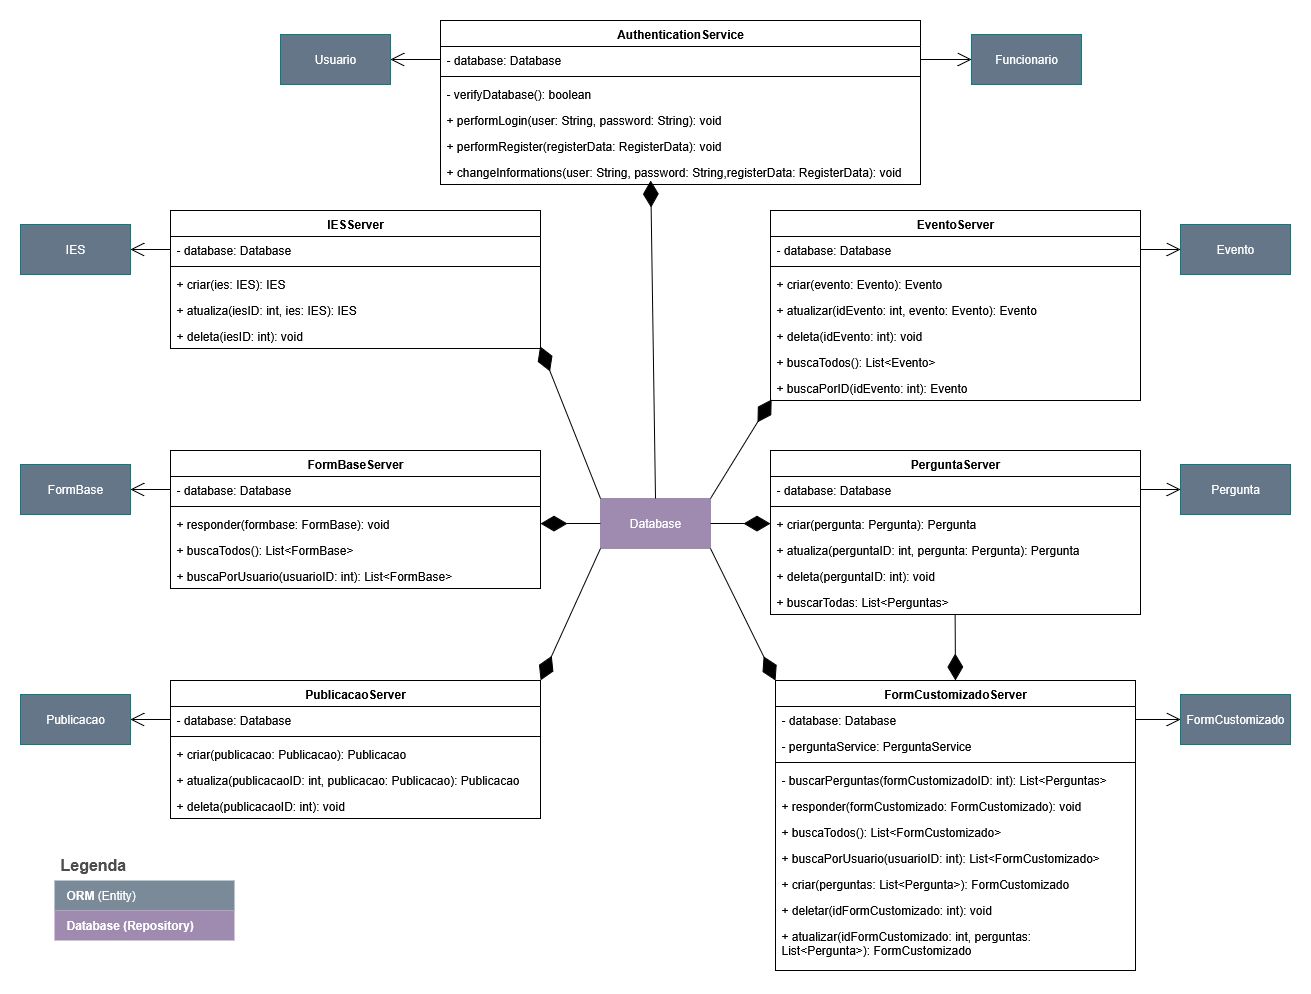
\includegraphics[width=0.55\textheight]{figuras/DIAGRAMA_CLASSE.png}
    \par
    Fonte: autoria própria com base em \citeonline{guedes2018}.
    \par
    \label{diaclasseprojeto}
\end{figure}


\subsection{Diagrama de Pacotes}

De certo, o diagrama de pacotes é a escolha ideal para demonstrar como os subsistemas ou submódulos interagem entre si. Ademais, uma das principais  utilidades está na demonstração das camadas de um software ou de um processo de desenvolvimento \cite{guedes2018}. Dessa forma, as Figuras~\ref{diapacfront} e ~\ref{diapacback} apresentam a estrutura em camadas dos módulos \textit{frontend} e \textit{backend}, respectivamente.

\begin{figure}[H]
    \centering
    \caption{Diagrama de Pacotes do frontend.}
    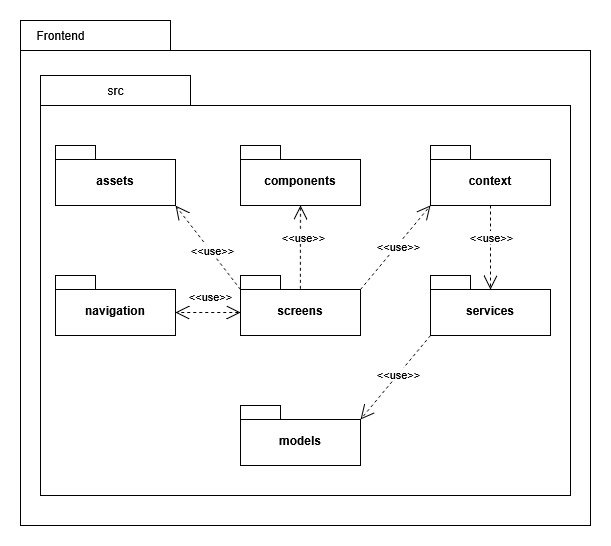
\includegraphics[height=0.55\textheight]{figuras/PACOTES_FRONT.png}
    \par
    Fonte: autoria própria com base em \citeonline{guedes2018}.
    \par
    \label{diapacfront}
\end{figure}

\begin{figure}[H]
    \centering
    \caption{Diagrama de Pacotes do backend.}
    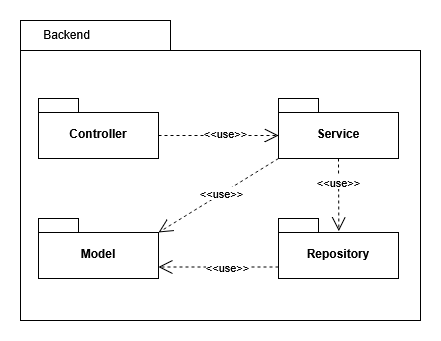
\includegraphics[height=0.4\textheight]{figuras/PACOTES_BACK.png}
    \par
    Fonte: autoria própria com base em \citeonline{guedes2018}.
    \par
    \label{diapacback}
\end{figure}